%%%%%%%%%%%%%%%%%%%%%%%%%%%%%%%%%%%%%%%%%
% Beamer Presentation
% LaTeX Template
% Version 1.0 (10/11/12)
%
% This template has been downloaded from:
% http://www.LaTeXTemplates.com
%
% License:
% CC BY-NC-SA 3.0 (http://creativecommons.org/licenses/by-nc-sa/3.0/)
%
%%%%%%%%%%%%%%%%%%%%%%%%%%%%%%%%%%%%%%%%%

%----------------------------------------------------------------------------------------
%	PACKAGES AND THEMES
%----------------------------------------------------------------------------------------

\documentclass[aspectratio=149]{beamer}
\usefonttheme[onlymath]{serif}


\mode<presentation> {

% The Beamer class comes with a number of default slide themes
% which change the colors and layouts of slides. Below this is a list
% of all the themes, uncomment each in turn to see what they look like.

\usetheme{default}
%\usetheme{AnnArbor}
%\usetheme{Antibes}
%\usetheme{Bergen}
%\usetheme{Berkeley}
%\usetheme{Berlin}
%\usetheme{Boadilla}
%\usetheme{CambridgeUS}
%\usetheme{Copenhagen}
%\usetheme{Darmstadt}
%\usetheme{Dresden}
%\usetheme{Frankfurt}
%\usetheme{Goettingen}
%\usetheme{Hannover}
%\usetheme{Ilmenau}
%\usetheme{JuanLesPins}
%\usetheme{Luebeck}
%\usetheme{Malmoe}
%\usetheme{Marburg}
%\usetheme{Montpellier}
%\usetheme{PaloAlto}
%\usetheme{Pittsburgh}
%\usetheme{Rochester}
%\usetheme{Singapore}
%\usetheme{Szeged}
%\usetheme{Warsaw}

% As well as themes, the Beamer class has a number of color themes
% for any slide theme. Uncomment each of these in turn to see how it
% changes the colors of your current slide theme.

%\usecolortheme{albatross}
\usecolortheme{beaver}
%\usecolortheme{beetle}
%\usecolortheme{crane}
%\usecolortheme{dolphin}
%\usecolortheme{dove}
%\usecolortheme{fly}
%\usecolortheme{lily}
%\usecolortheme{orchid}
%\usecolortheme{rose}
%\usecolortheme{seagull}
%\usecolortheme{seahorse}
%\usecolortheme{whale}
%\usecolortheme{wolverine}

%\setbeamertemplate{footline} % To remove the footer line in all slides uncomment this line
%\setbeamertemplate{footline}[page number] % To replace the footer line in all slides with a simple slide count uncomment this line

%\setbeamertemplate{navigation symbols}{} % To remove the navigation symbols from the bottom of all slides uncomment this line
}

\usepackage{graphicx} % Allows including images
\usepackage{booktabs} % Allows the use of \toprule, \midrule and \bottomrule in tables
\usepackage{verbatim}

\usepackage{mathtools} 
\usepackage{amssymb}
\usepackage{mathrsfs}
\usepackage{amsmath}
\usepackage{bm}

\usepackage{ragged2e}
\usepackage{etoolbox}
\usepackage{lipsum}

\usepackage{siunitx,booktabs}
\usepackage{pifont}
\usepackage{array}
\usepackage{tabu,booktabs}
\usepackage{tikz}
\usetikzlibrary{arrows,shapes}

\setbeamertemplate{enumerate items}[circle]
\usepackage{tikz}

\newcommand\mynum[1]{
  \usebeamercolor{enumerate item}
  \tikzset{beameritem/.style={circle,inner sep=0,minimum size=2ex,text=enumerate item.bg,fill=enumerate item.fg,font=\footnotesize}}%
  \tikz[baseline=(n.base)]\node(n)[beameritem]{#1};
}

\newcommand\mynumm[1]{
  \usebeamercolor{enumerate item}
  \tikzset{beameritem/.style={rectangle,inner sep=0,minimum size=2ex,text=enumerate item.bg,fill=enumerate item.fg,font=\footnotesize}}%
  \tikz[baseline=(n.base)]\node(n)[beameritem]{#1};
}

\def\Put(#1,#2)#3{\leavevmode\makebox(0,0){\put(#1,#2){#3}}}

\setbeamertemplate{footline}[]

%----------------------------------------------------------------------------------------
%	TITLE PAGE
%----------------------------------------------------------------------------------------

\title{ Subsidized Housing with Slum Externalities: \\ Evidence from South Africa } % The short title appears at the bottom of every slide, the full title is only on the title page

\author{Stefano Polloni \\
joint with Ben Bradlow and Will Violette} 

 % Your institution as it will appear on the bottom of every slide, may be shorthand to save space

\date{February 2017} %\today} % Date, can be changed to a custom date

\begin{document}

\beamertemplatenavigationsymbolsempty

\begin{frame}
\titlepage % Print the title page as the first slide
\end{frame}

%\begin{frame}
%\frametitle{Overview} % Table of contents slide, comment this block out to remove it
%\tableofcontents % Throughout your presentation, if you choose to use \section{} and \subsection{} commands, these will automatically be printed on this slide as an overview of your presentation
%\end{frame}

%----------------------------------------------------------------------------------------
%	PRESENTATION SLIDES
%----------------------------------------------------------------------------------------
\section{Introduction}
%------------------------------------------------

\begin{frame}
\frametitle{Slums and Development}

% In developing countries, 30\% of urban pop live in slums (UN, 2015)

\begin{itemize}
  \item Slum externalities $\rightarrow$ lasting poverty traps (Marx, 2013) 
    \begin{itemize}
      \item Overcrowding, poor infrastructure, high crime 
      \item Low investment in housing/public goods
    \end{itemize}  
\vspace{.2cm}
\pause
  \item \textbf{Public Housing} $\rightarrow$ primary government response
\end{itemize}
    \pause
\begin{enumerate}
  \item Direct Recipient Impacts
    \begin{itemize}
      \item Health, Wellbeing, Employment, Redistribution \\ \footnotesize{(Cateneo et al. [2009], Franklin et al. [2016], Galiani et al. [2017])}
    \end{itemize}
% ``key strategy for poverty alleviation'' {\footnotesize{South Africa}}
    \pause
    \vspace{.1cm}
\item Neighborhood Development
  \begin{itemize}
    \item ``combating crime, promoting social cohesion... spatial restructuring'' South Africa Dept. of Human Settlements
    \pause
    \item Little research on spillovers \footnotesize{(Diamond and McQuade (2016))}
  \end{itemize}
\end{enumerate}

\begin{itemize}
  \item \textbf{Question} \\ 
  \vspace{.1cm}
  What are the spillovers from public housing in developing contexts?
\end{itemize}
% ``combating crime, promoting social cohesion... spatial restructuring,'' {\footnotesize{South Africa}}
\end{frame}

%------------------------------------------------

\begin{frame}
\frametitle{This Paper}

\begin{itemize}
  \item \textbf{Question} \\ 
  \vspace{.1cm}
  What are the spillovers from public housing in developing contexts?
  \vspace{.1cm}
    \begin{itemize}
      \item \textbf{Positive:} Incentivize investments in housing/public goods
      \item \textbf{Negative:} Crowd in slum growth
    \end{itemize}

\pause
\vspace{1mm}
\item \textbf{Approach} \\ Leverage precise timing/geography of large housing projects
\vspace{1mm}
\item \textbf{New Data and Setting} \\ 172 projects in South Africa combined with GPS property transactions and slum growth data
\vspace{1mm}
\item \textbf{Initial Findings} \\ Housing projects depress home prices by 5\% within 300 meters
\begin{itemize}
  \item heterogeneity
  \item ballpark estimates
\end{itemize}
\end{itemize}

\end{frame}


%------------------------------------------------

\begin{frame}
\frametitle{Public Housing in South Africa}
  \begin{itemize}
      \item Over 4.3 million houses since 1994 (13\% of pop.)
%      \item Houses 13\% of the population
%      \item Single-story, two-room (30-40$\text{m}^2$) dwellings
      \begin{itemize}
        \item 50 to 500 houses per project
      \end{itemize}
  \end{itemize}
    %%% insert picture


\begin{itemize}
        \item Who gets a house?
      \begin{itemize}
        \item Official Policy: 
          \begin{itemize}
            \item National/provincial waiting lists
            \item No resale within 7 years
            \item Citizens, new homeowners, married or dependents, inc/month $<$R3,500
          \end{itemize}
        \item In Practice:
          \begin{itemize}
            \item Waiting lists/eligibility weakly enforced
            \item Only 82\% of houses occupied by initial owners within 5 yrs
          \end{itemize}
      \end{itemize}
\end{itemize}
\end{frame}

%------------------------------------------------

\begin{frame}
\frametitle{Where are these houses built?}

\begin{enumerate}
  \item \textbf{Greenfield projects} on undeveloped land near slums
  \item \textbf{In-Situ upgrading} replacing existing slums
\end{enumerate}

\begin{itemize}
  \item Projects are fully serviced (roads, water, sanitation, electricity)
\end{itemize}
    %%% insert small maps of pre-post periods (with cherry picked examples) (with google maps? or bblu?) or find good sattelite from an evaluation?

\end{frame}

%------------------------------------------------



\begin{frame}
\frametitle{Conceptual Framework: Public Housing Impacts}

\begin{enumerate}
  \item \textbf{Amenity Effect:} Upgrading housing stock/services
    \begin{itemize}
        \item Increase value of neighboring homes (Rossi-Hansberg [2010])
    \end{itemize}
\vspace{.2cm} 

  \item \textbf{Crowd-In Slums:} Reduce costs of informal housing
    \begin{itemize}
        \item Overburden services, health/crime externalities
        \item Reduce value of nearby houses
    \end{itemize}
\vspace{.2cm}

  \item \textbf{Demographic Effect:} New people in the neighborhood
    \begin{itemize}
        \item Taste-based discrimination (Diamond and McQuade [2016])
    \end{itemize}
\end{enumerate}

%\begin{enumerate}
%  \item Housing externalities  {\small (Rossi-Hansberg [2010]) }
%    \begin{itemize}
%      \item Home value depends on the quality of neighboring homes
%      \item ie. informal dwellings have poor sanitation
%    \end{itemize}
%\vspace{.1cm}
%  \item Demographic externalities
%    \begin{itemize}
%      \item Taste-based discrimination
%      \item Overcrowding $\rightarrow$ crime/health externalities
%    \end{itemize}
%\vspace{.1cm}
%  \item Access to public goods (water, sewer, road infrastructure)
%\end{enumerate}

\end{frame}



%------------------------------------------------



\begin{frame}
\frametitle{Measuring Public Housing and Spillovers}

\begin{itemize}
  \item Focus on Gauteng Province (includes Johannesburg and Pretoria)
\end{itemize}

\begin{enumerate}
\item \textbf{Property Transactions} measure housing projects and price impacts
  \begin{itemize}
    \item 500,000 deeds records (bottom 20\% of formal housing market)
    \item Buyer/seller name, GPS, price, date from 2002-2011
  \end{itemize}
\vspace{.2cm}
\item \textbf{Building Census} identifies slum-growth and in-situ upgrading
  \begin{itemize}
    \item 4 mil. residential buildings (50\% informal) GPS in 2001 and 2011
  \end{itemize}
\vspace{.2cm}
\item \textbf{Population Census} measures demographic and economic impacts
  \begin{itemize}
    \item Full census for 18,000 census blocks in 2001 and 2011
  \end{itemize}
\vspace{.2cm}
\item \textbf{Administrative Data} map projects (construction dates and costs)
  \begin{itemize}
    \item Not comprehensive
    \item Includes planned but unconstructed projects
  \end{itemize}


\end{enumerate}

\end{frame}

%------------------------------------------------

%  
%  
%  \item \textbf{Temporal Clustering:} include cluster with $>$50\% of transactions during modal year


\begin{frame}
\frametitle{Identifying Housing Projects}

\begin{tikzpicture}[overlay]

\onslide<1->\node[overlay,anchor=west,align=left] at (0, 2.5) {    \begin{minipage}{1\textwidth} {\begin{enumerate}
  \item \textbf{Seller Identity:} match government names and housing authorities in seller-names from transactions 
\end{enumerate}}\end{minipage}};

\onslide<2->\node[overlay,anchor=west,align=left] at (0, 1.5) {    \begin{minipage}{1\textwidth} { 
\begin{enumerate}
  \setcounter{enumi}{1}
  \item \textbf{Subsidy Value:} exclude purchase prices R50,000 above subsidy value
\end{enumerate}}\end{minipage}};

\onslide<3->\node[overlay,anchor=west,align=left] at (0, .5) {    \begin{minipage}{1\textwidth} { 
\begin{enumerate}
  \setcounter{enumi}{2}
  \item \textbf{Pre-Existing Formal Dwellings:} exclude land plots with formal structures in 2001 building census
\end{enumerate}}\end{minipage}};

\onslide<4->\node[overlay,anchor=west,align=left] at (0, -.5) {    \begin{minipage}{1\textwidth} { 
\begin{enumerate}
  \setcounter{enumi}{3}
  \item \textbf{Spatial Clustering:} collect nearby houses into projects with density-based clustering algorithm
\end{enumerate}}\end{minipage}};

\onslide<5->\node[overlay,anchor=west,align=left] at (0, -1.5) {    \begin{minipage}{1\textwidth} { 
\begin{enumerate}
  \setcounter{enumi}{4}
  \item \textbf{Temporal Clustering:} include clusters with $>$50\% of transactions during modal year
\end{enumerate}}\end{minipage}};

\onslide<5->\node[overlay,anchor=west,align=left] at (0, -2.6) {    \begin{minipage}{1\textwidth} { 
\begin{itemize}
  \item Overlaps well with completed projects from admin. data
\end{itemize}}\end{minipage}};



\onslide<1>\node[overlay,anchor=west,align=left] at (0, -1) {
\begin{minipage}{1\textwidth} { 
\begin{figure}
\caption{Top 5 Seller Names}
\begin{tabu}{lc}
\toprule
 Seller Name & Observations \\
\midrule
City Of Johannesburg Metropolitan Municipality & 29,087  \\
City Of Johannesburg & 27,672  \\
City Of Tshwane Metropolitan Municipality & 24,780  \\
Ekurhuleni Metropolitan Municipality & 21,758  \\
Gauteng Provincial Housing Advisory Board & 13,058  \\
{\bf Total Observations }& {\bf 549,704}  \\
\bottomrule
\end{tabu}
 
\end{figure}
}\end{minipage}
} ;

\onslide<2>\node[overlay,anchor=west,align=left] at (0, -1.7) { 
\begin{minipage}{1\textwidth} { 
\begin{figure}
\caption{Purchase Price Densities}
 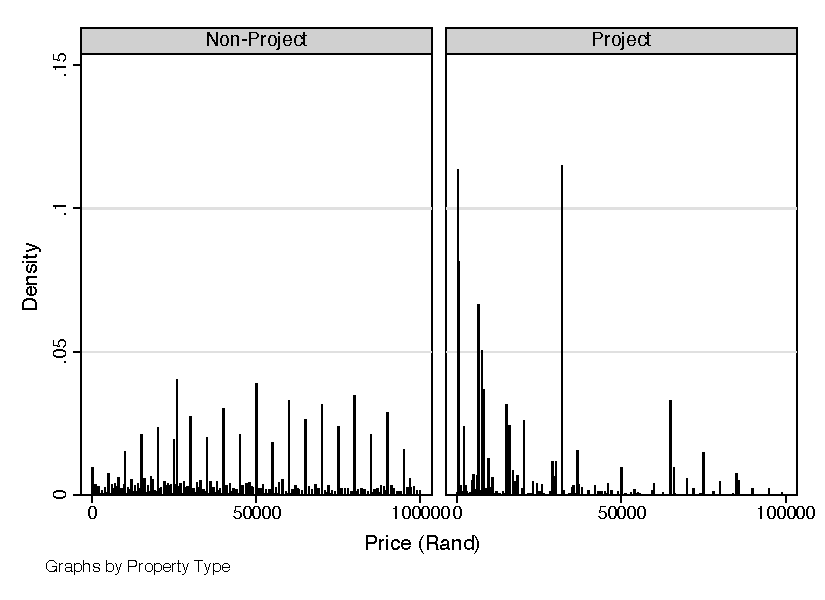
\includegraphics[scale=.53]{price_histogram.pdf} 
\end{figure}
}\end{minipage} 
} ;

\onslide<4>\node[overlay,anchor=west,align=left] at (2, -2.8) {  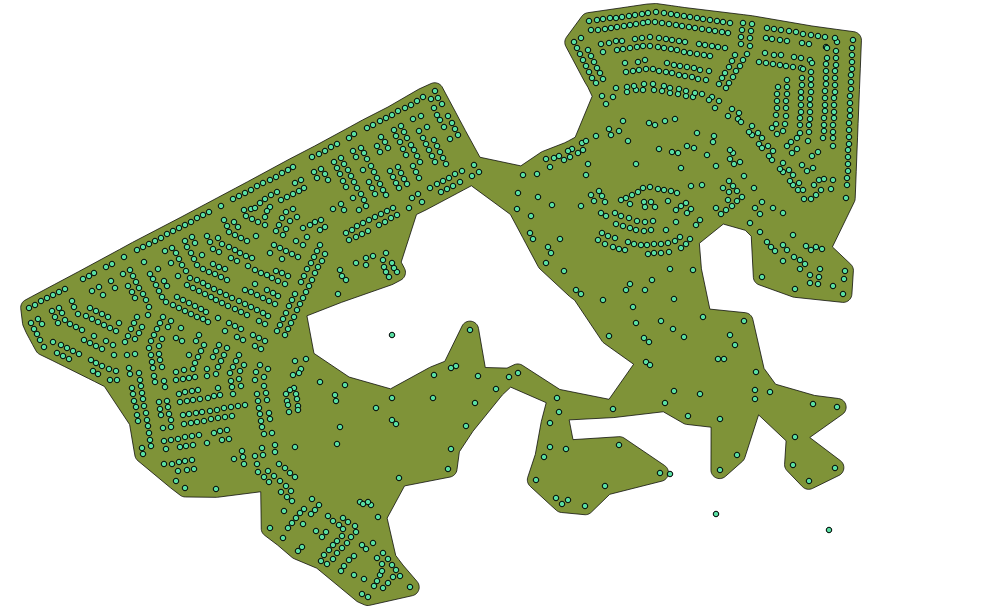
\includegraphics[scale=.16]{rdp_conhull_pic.png}  };


\end{tikzpicture}

\end{frame}





%------------------------------------------------


\begin{frame}
\frametitle{Identifying Planned but Unconstructed Projects}

\begin{enumerate}
  \item Admin. data have ``planned,'' ``proposed,'' ``implementing'' projects
    \begin{itemize}
      \item Exclude projects with identified project transactions
    \end{itemize}

    \vspace{.2cm}

  \item Assign projects an expected completion date
    \begin{itemize}
      \item Fuzzy-string match budget data (with start-dates) on project names
      \item Add avg. diff. between transaction-date and start-date for completed projects
    \end{itemize}
\end{enumerate}

\begin{itemize}
  \item Why are projects canceled/delayed? 
    \begin{itemize}
      \item Legal disputes, service delivery backlogs, funding complications
      \item Delays often exceed 12 years 
    \end{itemize} 
\end{itemize}

\end{frame}


%------------------------------------------------

\begin{frame}
\frametitle{Housing Projects}
\begin{table}
\caption{Housing Projects and Building Growth}
\begin{tabu}{lcc}
 & Completed & Uncompleted \\ 
 Formal Density: 2001  & 340.6  & 89.1  \\ 
 Formal Density: 2011  & 1,783.1  & 491.1  \\ 
 &  &  \\ 
 Informal Density: 2001  & 443.0  & 1,569.2  \\ 
 Informal Density: 2011  & 1,064.6  & 1,993.4  \\ 
 &  &  \\ 
 Median Year (est.)  & 2005  & 2007  \\ 
 Distance to CBD (km)  & 28.9  & 27.6  \\ 
 &  &  \\ 
 Total Projects   & 56  & 35  \\ 
\bottomrule
\end{tabu}

\end{table}
\vspace{.2cm} 
Density is building number per square kilometer.
\end{frame}

%------------------------------------------------

\begin{frame}
\frametitle{Measure outcomes in close neighborhoods}
\begin{itemize}
  \item Focus on 1.2 km buffers around housing projects
\end{itemize}

\begin{center}
\begin{figure}
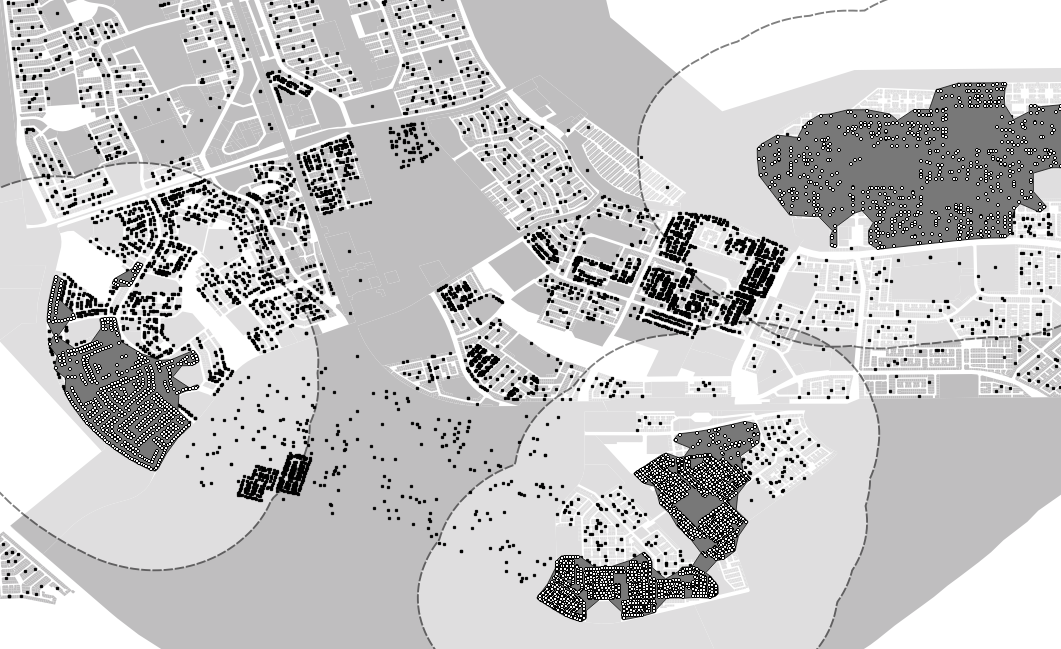
\includegraphics[scale=0.30]{design2.png}
\vspace{-3mm}
\end{figure}
\end{center}

\end{frame}

%------------------------------------------------

\begin{frame}
\frametitle{Using deeds data to estimate RDP impact on housing prices}

\begin{center}
\begin{figure}
%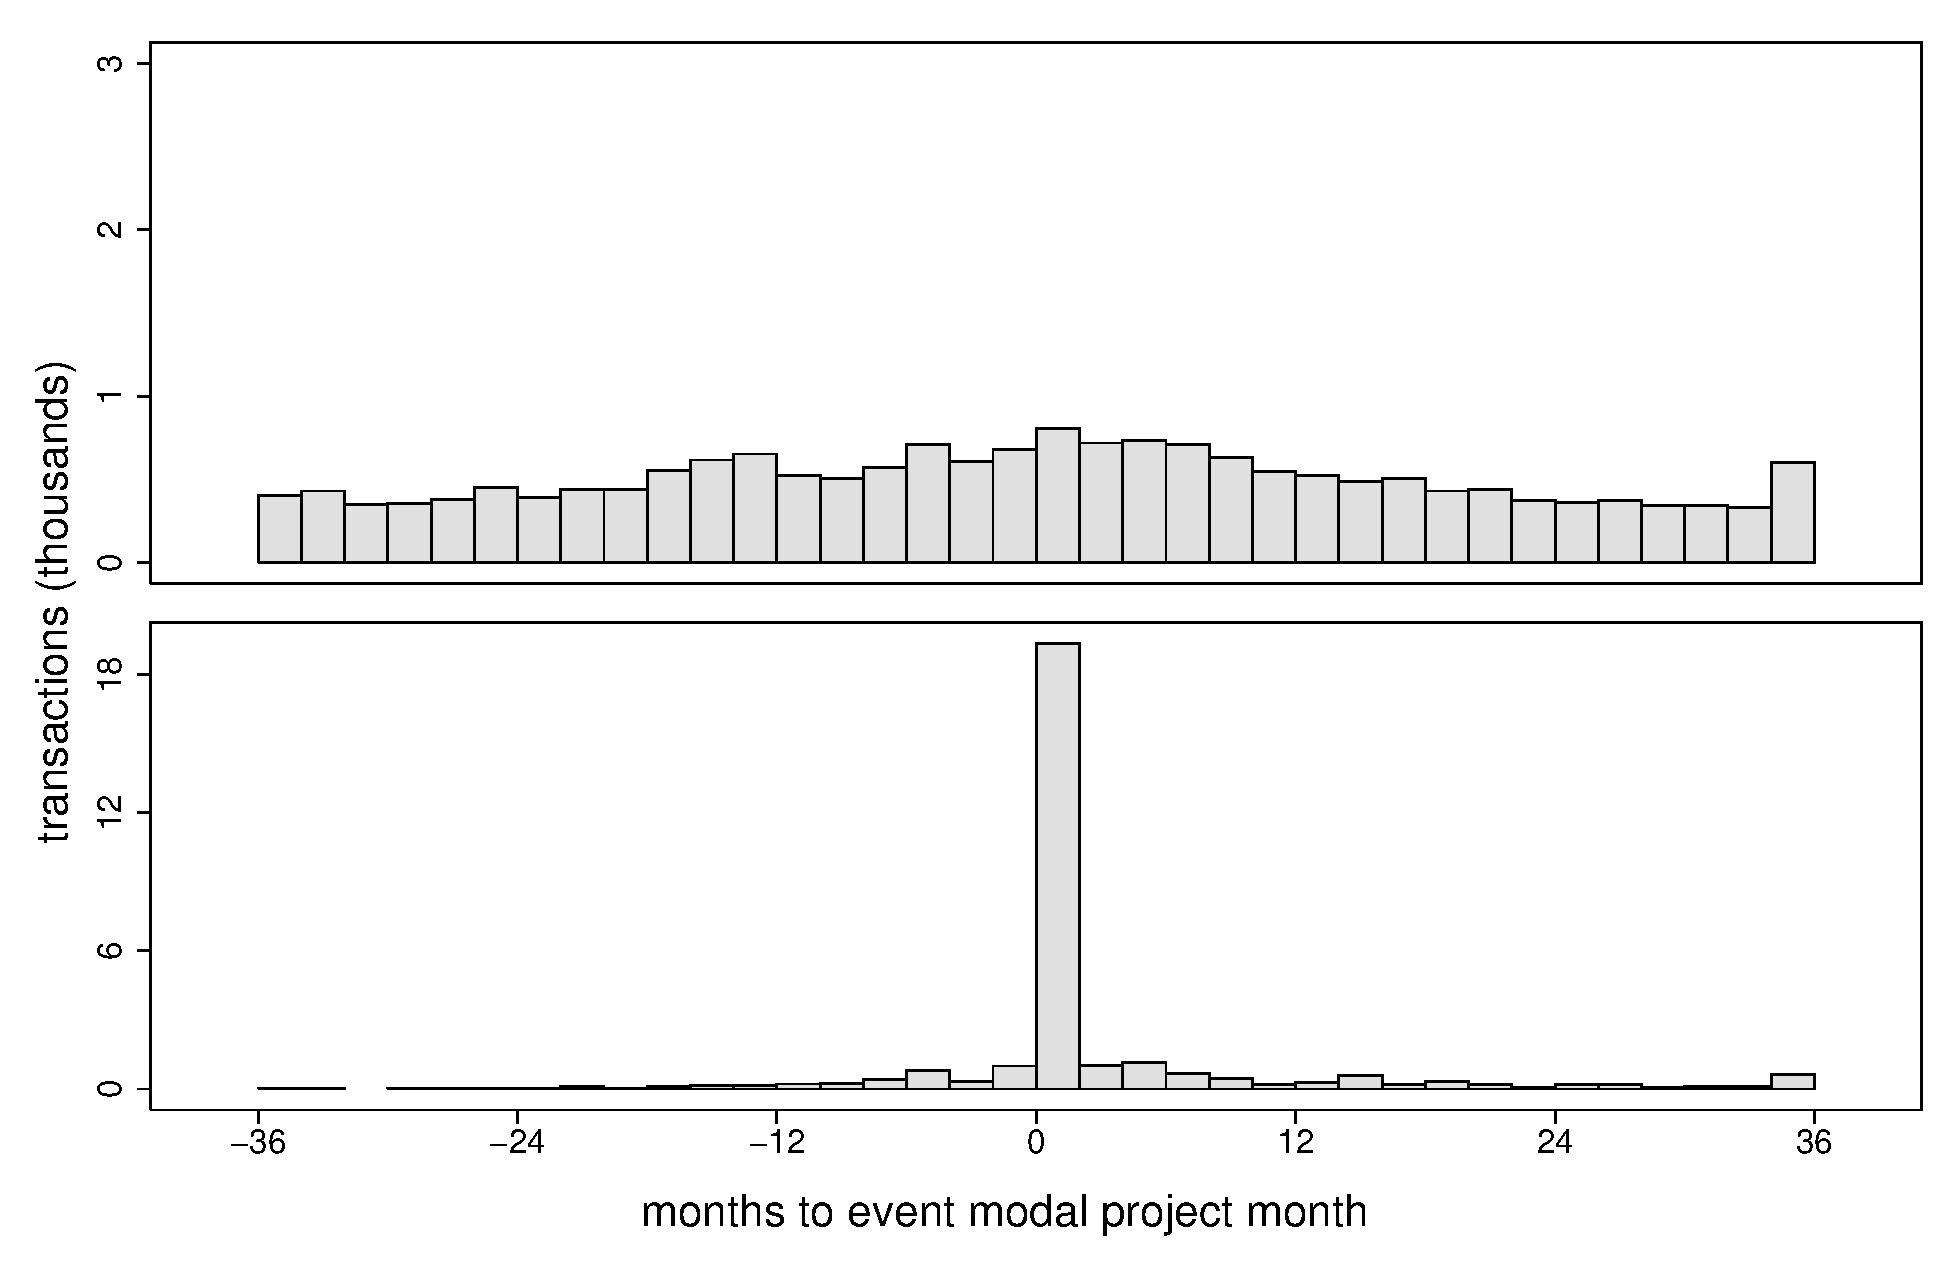
\includegraphics[scale=0.65]{summary_densitytime.pdf}
\vspace{-3mm}
\caption{density of RDP vs Non-Rdp transactions centered around "event month"}
\end{figure}
\end{center}


\end{frame}

%------------------------------------------------

\begin{frame}
\frametitle{Using deeds data to estimate RDP impact on housing prices}

\begin{center}
\begin{figure}
%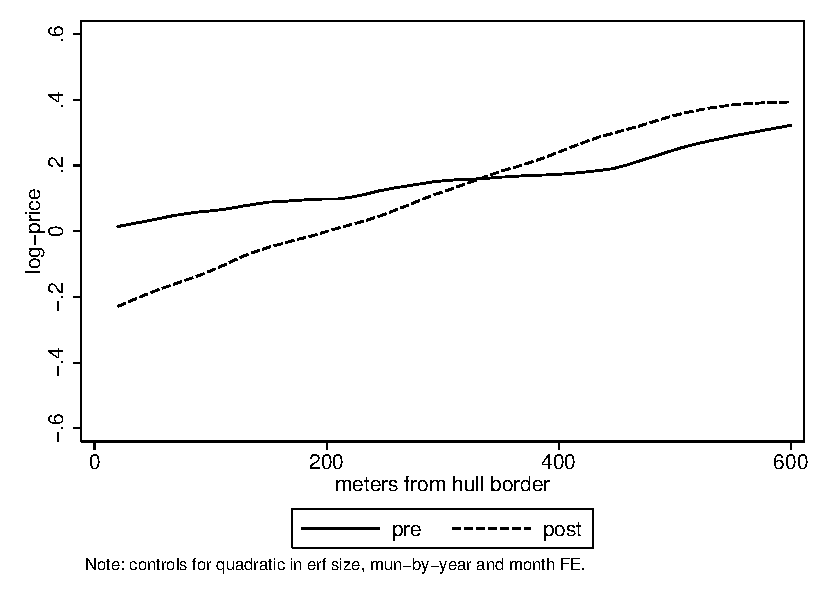
\includegraphics[scale=0.65]{reg_pm1.pdf}
\vspace{-3mm}
\caption{Smoothed distance dummy coefficients of log-price of Non-RDP transactions, before and after mode year of construction.}
\end{figure}
\end{center}


\end{frame}

%------------------------------------------------

\begin{frame}
\frametitle{Using deeds data to estimate RDP impact on housing prices}

\begin{center}
\begin{figure}
%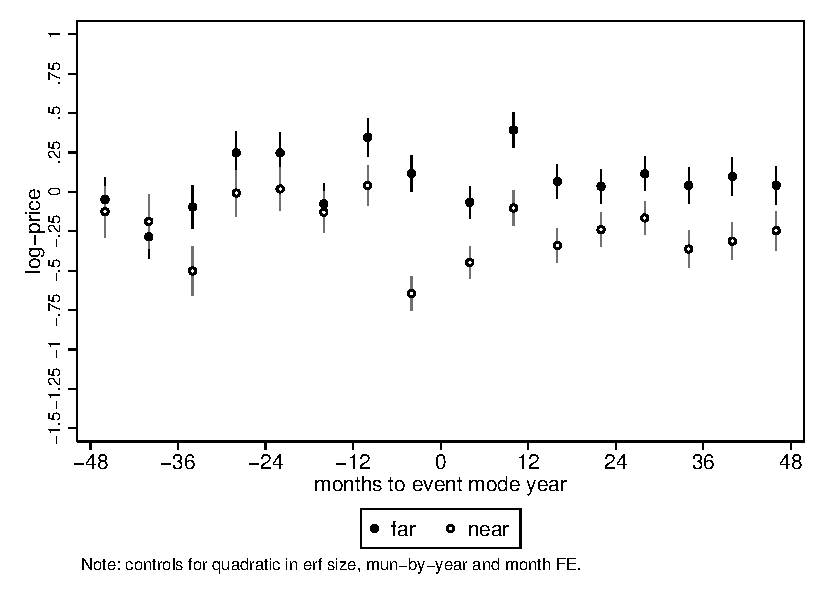
\includegraphics[scale=0.65]{timereg_pm1.pdf}
\vspace{-3mm}
\caption{6-month dummy coefficients of log-price of Non-RDP transactions, $<$300m (near) and $>$300m (far) from border of RDP project.}
\end{figure}
\end{center}


\end{frame}

%------------------------------------------------



\begin{frame}
\frametitle{A Model of Housing with Slum Externalities}

Basic Setup:
\vspace{2mm}
\begin{itemize}
  \item A city is comprised of $N$ residential neighborhoods indexed $n\in\{1,...,N\}$. 
  \vspace{2mm}
  \item Each neighborhood has a formal and informal housing sector, indexed $s\in\{F,I\}$.
  \vspace{2mm}
  \item All jobs are in the CBD and pay a fixed wage rate; commuting to the CBD is costly.
\end{itemize}


\end{frame}

%------------------------------------------------

\begin{frame}
\frametitle{Housing Demand}

Housing Demand:
\vspace{2mm}
\begin{itemize}
  \item Measure one of freely-mobile agents inelastically demand one unit of housing.
  \vspace{2mm}
  \item An agent $i$ has idiosyncratic tastes for neighborhoods, represented by the vector $\bm{\epsilon}_i \in \mathbb{R}^{2N}$ of neighborhood-sector specific valuations.
  \vspace{2mm}
  \item The distribution of preferences in the population is given by density $f(\bm{\epsilon})$ such that $\int f(\bm{\epsilon}) d\bm{\epsilon} = 1$.
\end{itemize}


\end{frame}

%------------------------------------------------

\begin{frame}
\frametitle{Housing Demand}

Indirect Utility:

\begin{equation*}
\begin{aligned}
u_{ins} \,& =\, A_n\,+\, B_s - R_{ns} \,+\, \epsilon_{ins} \\
        \,& =\, v_{ns} \,+\, \epsilon_{ins}
\end{aligned}
\end{equation*}

With:
\vspace{2mm}
\begin{itemize}
  \item $A_n$ is net-of-commuting and amenity-adjusted wage received in $n$.
  \item $B_s$ is a utility component specific to living in sector $s$
  \item $R_{ns}$ is the rental rate of housing.
  \item $\epsilon_{ins}$ is individual $i$'s taste for neighborhood-sector pair $(n,s)$.
\end{itemize}

\vspace{5mm}

Individual $i$ takes exogenous quantities $\{\bm{A},\bm{B},\bm{\epsilon}_i\}$ and endogenous rents $\bm{R}$ as given, and locates in pair $(n,s)$ yielding the highest indirect utility.


\end{frame}

%------------------------------------------------

\begin{frame}
\frametitle{Housing Demand}

Aggregate housing demand $H_{ns}$ in $(n,s)$ given by:

\begin{equation*}
\begin{aligned}
H_{ns} \,\,& =\,\, \int I\Big( \, u_{ins} \,=\, \max_{n's'}\{u_{in' s'} \,\,|\,\, \bm{A},\bm{B},\bm{R}\,\} \Big)f(\bm{\epsilon}) d\bm{\epsilon}    \\[.2em]
        \,\,& =\,\, D_{ns}(\bm{A},\bm{B},\bm{R})
\end{aligned}
\end{equation*}

\end{frame}

%------------------------------------------------

\begin{frame}
\frametitle{Housing Supply}

\begin{itemize}
  \item Neighborhoods are endowed with $L_n$ units of land.
  \item A share $\theta_{nF}$ of the total land stock is available for formal residential development, while the rest, $\theta_{nI} = 1-\theta_{nF}$, is vacant or public land suited for informal housing.
  \item Price-taking landlords supply housing by combining land and materials $M$ with CRS technology $q(L,M)$.
  \item Materials are supplied at fixed cost $c$ on a large national market.
  \item Government can subsidize housing in market $(n,s)$ at a rate of $\delta_{ns}$ per unit.
\end{itemize}

Because land is fixed in every market, the marginal cost of housing is increasing. The inverse supply curve in $(n,s)$ is:

\begin{equation*}
R_{ns} \,\, =\,\, S(H_{ns},\theta_{ns}L_n) - \delta_{ns}
\end{equation*} 

\vspace{4mm}

\end{frame}

%------------------------------------------------

\begin{frame}
\frametitle{Equilibrium}
{\small
Given density $f(\bm{\epsilon})$ and exogenous quantities $\{\bm{A},\bm{B},\bm{L},\bm{\theta}\}$, an equilibrium consists of rents $\bm{R}^*$ and housing quantities $\bm{H}^*$ such that all housing markets clear, that is, $\forall (n,h)$:

\begin{equation*}
\begin{aligned}
& H^*_{ns} \,\, =\,\, D_{ns}(\bm{A},\bm{B},\bm{R}^*) \\
\text{and}\quad & R^*_{ns} \,\, =\,\, S(H^*_{ns},\theta_{ns}L_n) - \delta_{ns} \text{,}
\end{aligned}
\end{equation*} }


\noindent and all agents live somewhere: $\sum_{n}\sum_{s} H^*_{ns} = 1$

\begin{center}
\begin{figure}
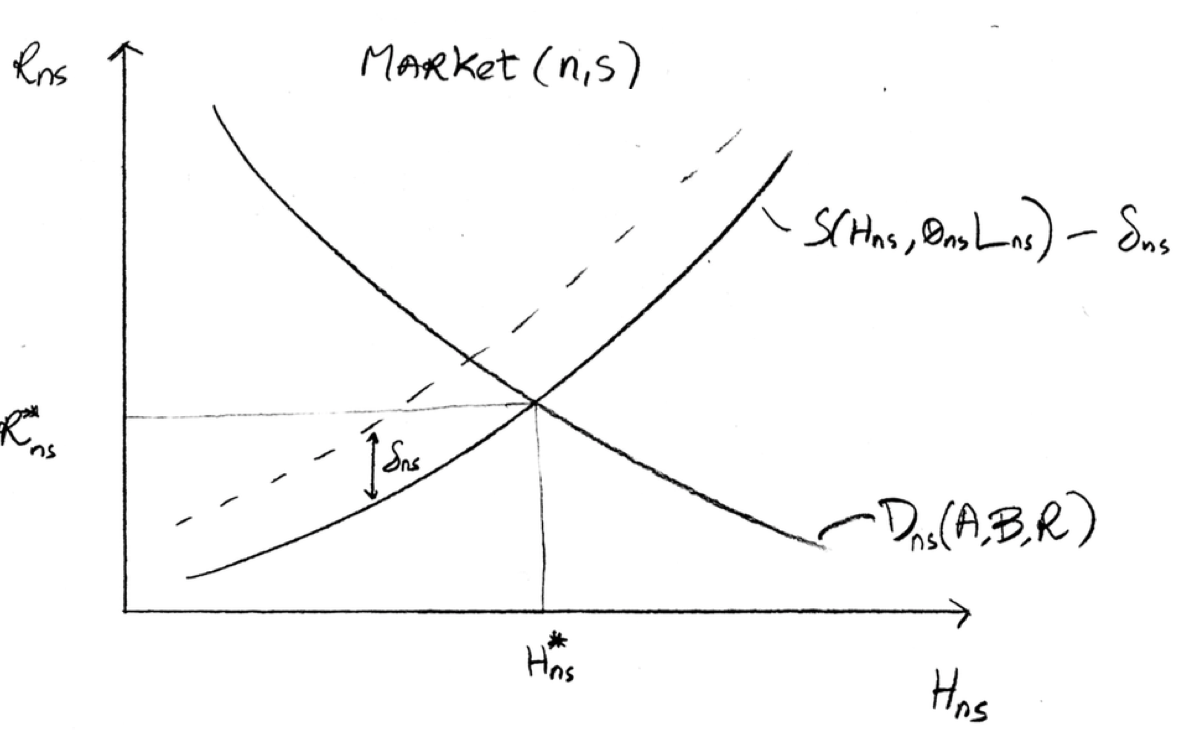
\includegraphics[scale=0.16]{market.png}
\vspace{-3mm}
\end{figure}
\end{center}


\end{frame}

%------------------------------------------------

\begin{frame}
\frametitle{Welfare}

The sum of individuals' utility is given by:

\begin{equation*}
U \,\, =\,\, \int \max_{n's'}\{u_{in' s'}\,\,|\,\, \bm{A},\bm{B},\bm{R}^*\,\}f(\bm{\epsilon}) d\bm{\epsilon} 
\end{equation*}

\vspace{3mm}

\noindent and total landlords' profit is:

\begin{equation*}
\Pi \,\, =\,\, \sum_{n}\sum_{s} \Bigg(\,\int_0^{H^*_{ns}} [R^*_{ns} - (S(x,\theta_{ns}L_n) - \delta_{ns})]dx \, \Bigg) 
\end{equation*} 

\vspace{3mm}

Total social welfare is:

\begin{equation*}
W = U + \Pi
\end{equation*} 

\end{frame}

%------------------------------------------------

\begin{frame}
\frametitle{Welfare Implications of Subsidies (No Market Failures)}

We are interested in the welfare implications of the government subsidizing formal housing in a subset $\mathcal{N}\subset\{1,...,N\}$ of neighborhoods:

\vspace{2mm}

\begin{equation*}
 \delta_{ns} = \begin{cases} 
      \,\,\delta & \text{if}\,\, n\in\mathcal{N} \,\,\text{and}\,\, $s=F$ \\
      \,\,0 & \text{otherwise} 
   \end{cases}
\end{equation*} 

\vspace{2mm}

After some algebra, we can show that the marginal welfare effect of changing $\delta$ simplifies to: 

\vspace{2mm}

\begin{equation*}
\frac{\partial W}{\partial\delta} \,\,=\,\, \frac{\partial U}{\partial\delta} \,\,+\,\, \frac{\partial \Pi}{\partial\delta} \,\,=\,\, \sum_{n\in\mathcal{N}} H^*_{nF}
\end{equation*} 


\end{frame}

%------------------------------------------------

\begin{frame}
\frametitle{Welfare Implications of Subsidies (No Market Failures)}

The total cost of the subsidy is given by $TC = \sum_n\sum_s H^*_{ns}\delta_{ns}$ and its marginal cost is therefore:
\begin{equation*}
 \frac{\partial TC}{\partial \delta} \,\,=\,\, \sum_{n\in\mathcal{N}} \Big( H^*_{nF} \,\,+\,\, \delta\frac{\partial H^*_{nF}}{\partial \delta} \Big)
 \end{equation*} 

 \vspace{1mm}

 The extra term in this expression relative to (2) represents the marginal deadweight loss from an increase in $\delta$. The magnitude of the inefficiencies depends on the population responses in subsidized markets, $\frac{\partial H^*_{nF}}{\partial \delta}$.

\end{frame}

%------------------------------------------------

\begin{frame}
\frametitle{Welfare Implications with Slum Externalities}

We consider an external utility cost from informal housing of the form:

\begin{equation*}
A_n \,\,=\,\, \bar{A}_n \,\,+\,\, a\Big(\frac{H_{nI}}{L_n}\Big)
\end{equation*} 


where $a'(.)<0$. The private decision of locating in $(n,I)$ negatively impacts all residents in $n$ because of congestion effects. The welfare response to $\delta$ is now:

\begin{equation*}
\frac{\partial W}{\partial\delta} \,\,=\,\, \sum_{n\in\mathcal{N}} H^*_{nF} \,\,+\,\, \sum_{n} \underbracket{a'\Big(\frac{H^*_{nI}}{L_n}\Big)}_{(<0)}\,\underbracket{\frac{\partial H^*_{nI}}{\partial \delta}}_{(<0)}\,\frac{(H^*_{nF}+H^*_{nI})}{L_n}
\end{equation*}

The subsidy $\delta$ makes formal housing in $\mathcal{N}$ more attractive relative to informal housing. Marginal residents moving to $\mathcal{N}$ make remaining residents better-off because of reduced congestion.

\end{frame}

%------------------------------------------------

\begin{frame}
\frametitle{Welfare Implications with Slum Externalities}

Since the cost of the subsidy is unaffected by the externality, the marginal deadweight loss is now:

\begin{equation*}
\begin{aligned}
MDWL \,\,&=\,\, \frac{\partial TC}{\partial \delta} - \frac{\partial W}{\partial \delta} \\[.6em]
     \,\,&=\,\, \sum_{n\in\mathcal{N}} \,\delta\frac{\partial H^*_{nF}}{\partial \delta} \,\,-\,\, \sum_{n} \, a'\Big(\frac{H^*_{nI}}{L_n}\Big)\,\frac{\partial H^*_{nI}}{\partial \delta}\,\frac{(H^*_{nF}+H^*_{nI})}{L_n} \\
\end{aligned}
\end{equation*}

 $\delta=0$ implies $MDWL<0$. Some level of subsidy $\delta$ is welfare improving when compared to no subsidy. This is expected since the social benefits exceed the private benefits of moving from informal to formal housing. 

\end{frame}


%------------------------------------------------

\begin{frame}
\frametitle{Welfare with Slum Externalities and Subsidy Spillovers.}

To capture the possibility of increased "backyarding", we now assume subsidies in the formal sector spillover to the informal sector at no additional cost for the government:

\begin{equation*}
 \delta_{ns} = \begin{cases} 
      \,\,\delta & \text{if}\,\, n\in\mathcal{N} \,\,\text{and}\,\, $s=F$ \\
      \,\,\alpha\delta & \text{if}\,\, n\in\mathcal{N} \,\,\text{and}\,\, $s=I$ \\
      \,\,0 & \text{otherwise} 
   \end{cases}
\end{equation*}

This yields:

\begin{equation*}
\frac{\partial W}{\partial\delta} \,\,=\,\, \sum_{n\in\mathcal{N}} \big( H^*_{nF} + \alpha H^*_{nI} \big)  \,\,+\,\, \sum_{n} \underbracket{a'\Big(\frac{H^*_{nI}}{L_n}\Big)}_{(<0)}\,\underbracket{\frac{\partial H^*_{nI}}{\partial \delta}}_{(\lessgtr0)}\,\Big(\frac{H^*_{nF}+H^*_{nI}}{L_n} \Big)
\end{equation*} 

\end{frame}


%------------------------------------------------

\begin{frame}
\frametitle{Welfare with Slum Externalities and Subsidy Spillovers.}

The presence of such spillovers alter welfare implications in two ways:

\begin{itemize}
  \item Suppliers of informal housing benefit from an increase in profit due to the indirect subsidies.
  \item For $n\in\mathcal{N}$, the sign of informal housing response $\frac{\partial H^*_{nI}}{\partial\delta}$ is now ambiguous and depends on the magnitude of $\alpha$.\footnote{ This can also be shown formally by combining the equilibrium conditions in (1) and using the implicit function theorem. For $n\in\mathcal{N}^C$, $\frac{\partial H^*_{nI}}{\partial\delta}$ remains unambiguously negative.} When $\alpha$ is large, the indirect subsidies in $(n,I)$ dominate and net-migration is positive, i.e. $\frac{\partial H^*_{nI}}{\partial\delta}>0$, making incumbent residents in $(n,I)$ and $(n,F)$ worse-off.
\end{itemize}

\end{frame}

%------------------------------------------------

\begin{frame}
\frametitle{Takeaways from the model}

With this set-up, welfare considerations depend critically on 3 quantities:

\vspace{2mm}

\begin{itemize}
  \item The shape of externalities $a(\,)$ -- this is research question {\!\!\!\mynum{1}}.
  \vspace{1mm}
  \item The extent of spillovers $\alpha$ -- this is research question {\!\!\!\mynum{2}}.
  \vspace{1mm}
  \item The population (housing) responses in both subsidized formal markets, $\frac{\partial H^*_{nF}}{\partial \delta}\,\,\forall n\in\mathcal{N}$,  and informal markets, $\frac{\partial H^*_{nI}}{\partial \delta}\,\,\forall n$.
\end{itemize}

\end{frame}







\end{document} 
